\subsection{Glass Tile}
\paragraph{Korrektheit}
Die Korrektheit der Implementierung des portierten Algorithmus wurde mithilfe der Gegl-Testumgebung geprüft mit dem Ergebnis, dass für verschieden gewählte Parameter stets eine Übereinstimmung mit dem GIMP-Referenzbild besteht.

\paragraph{Laufzeit}
Das Testsystem ist ein Intel Core-2-Duo 2,2 GHz Notebook mit zwei Kernen und 2GB RAM. Als Testbild wurde ein 5000x3450 Pixel großes png-Bild mit 21 MB Dateigröße verwendet.
%Es wurden jeweils 50 Testläufe durchgeführt.
Als Umgebungsvariablen für Gegl wurden die Default-Werte verwendet. Für die detaillierte Ansicht der einzelnen Gegl-Aufrufe und die zugehörige Zeitmessung wurde die \emph{GEGL\_DEBUG\_TIME} auf \emph{TRUE} gesetzt. Wie in Abbildung~\ref{fig:gtile-dias} zu sehen ist, benötigt die parallele Version länger als die sequentielle Version, was bereits weiter oben angedeutet wurde. Die sequentielle Variante gegl:tile-glass-seq wird in 0,73 sek ausgeführt, wohingegen die parallele Version mit 2 Threads gegl:tile-glass in 0,85 sek läuft.

\begin{figure}[h]
\begin{center}
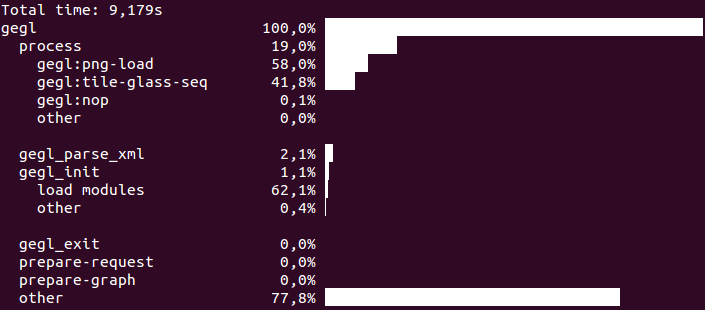
\includegraphics[width=1.0\textwidth]{gtile_seq_dia.png}
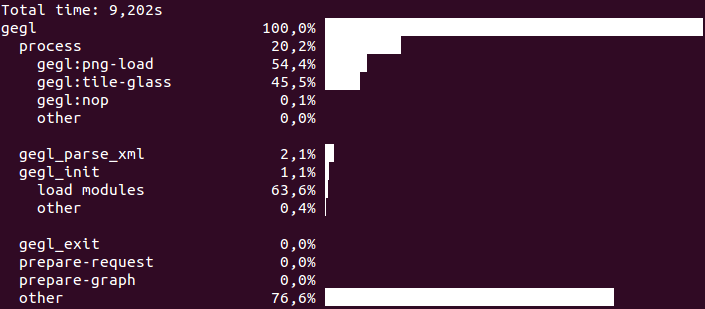
\includegraphics[width=1.0\textwidth]{gtile_par_dia.png}
\end{center}
\caption{Detailansicht der Gegl-Aufrufe (sequ. Variante oben, parallele Variante mit 2 Threads unten)}\label{fig:gtile-dias}
\end{figure}
%X Durchläufe in Diagram abtragen?
%System beschreiben (Hardware, Software, Umgebungsvariablen) !!!
%Boxplots !!!
%Statistische Analyse ?!
%Aus Debug-Output Diagramm erstellen um Anteil des Filters an Gesamtlaufzeit zu verdeutlichen